\documentclass[10pt]{article}
\usepackage[a4paper,landscape,margin=0pt]{geometry}
\usepackage{graphicx}
\usepackage{tikz}
\usepackage{xcolor}
\usepackage[T1]{fontenc}
\usepackage[utf8]{inputenc}
\pagestyle{empty}
\setlength{\parindent}{0pt}

% =============================================================================
% Carte de Chult - feuille A4 paysage
% Gauche : carte de Chult
% Droite : légende sur fond parchemin
%
% Coordonnées normalisées des marqueurs :
% x = 0 bord gauche ; x = 1 bord droit
% y = 0 bord bas    ; y = 1 bord haut
% =============================================================================

\definecolor{markerred}{HTML}{A52A2A}
\definecolor{markertext}{HTML}{2B2118}

% Chaque moitié fait exactement 148.5 x 210 mm.
\newcommand{\MapX}{0}
\newcommand{\MapY}{0}
\newcommand{\MapW}{148.5}
\newcommand{\MapH}{210}

\newcommand{\MapMarker}[3]{%
  \pgfmathsetmacro{\mx}{\MapX + (#2)*\MapW}%
  \pgfmathsetmacro{\my}{\MapY + (#3)*\MapH}%
  \node[
    circle,
    fill=markerred,
    draw=white,
    line width=0.7pt,
    minimum size=6.8mm,
    inner sep=0pt,
    font=\bfseries\small,
    text=white
  ] at ([xshift=\mx mm,yshift=\my mm]current page.south west) {#1};%
}

\newcommand{\LegendNumber}[1]{%
  \tikz[baseline=(n.base)]\node[
    circle,
    fill=markerred,
    draw=markertext,
    line width=0.45pt,
    minimum size=6.5mm,
    inner sep=0pt,
    font=\bfseries\small,
    text=white
  ] (n) {#1};%
}

\begin{document}
\begin{tikzpicture}[remember picture,overlay,x=1mm,y=1mm]

  % Carte de Chult - moitié gauche.
  \node[anchor=south west,inner sep=0pt]
    at (current page.south west)
    {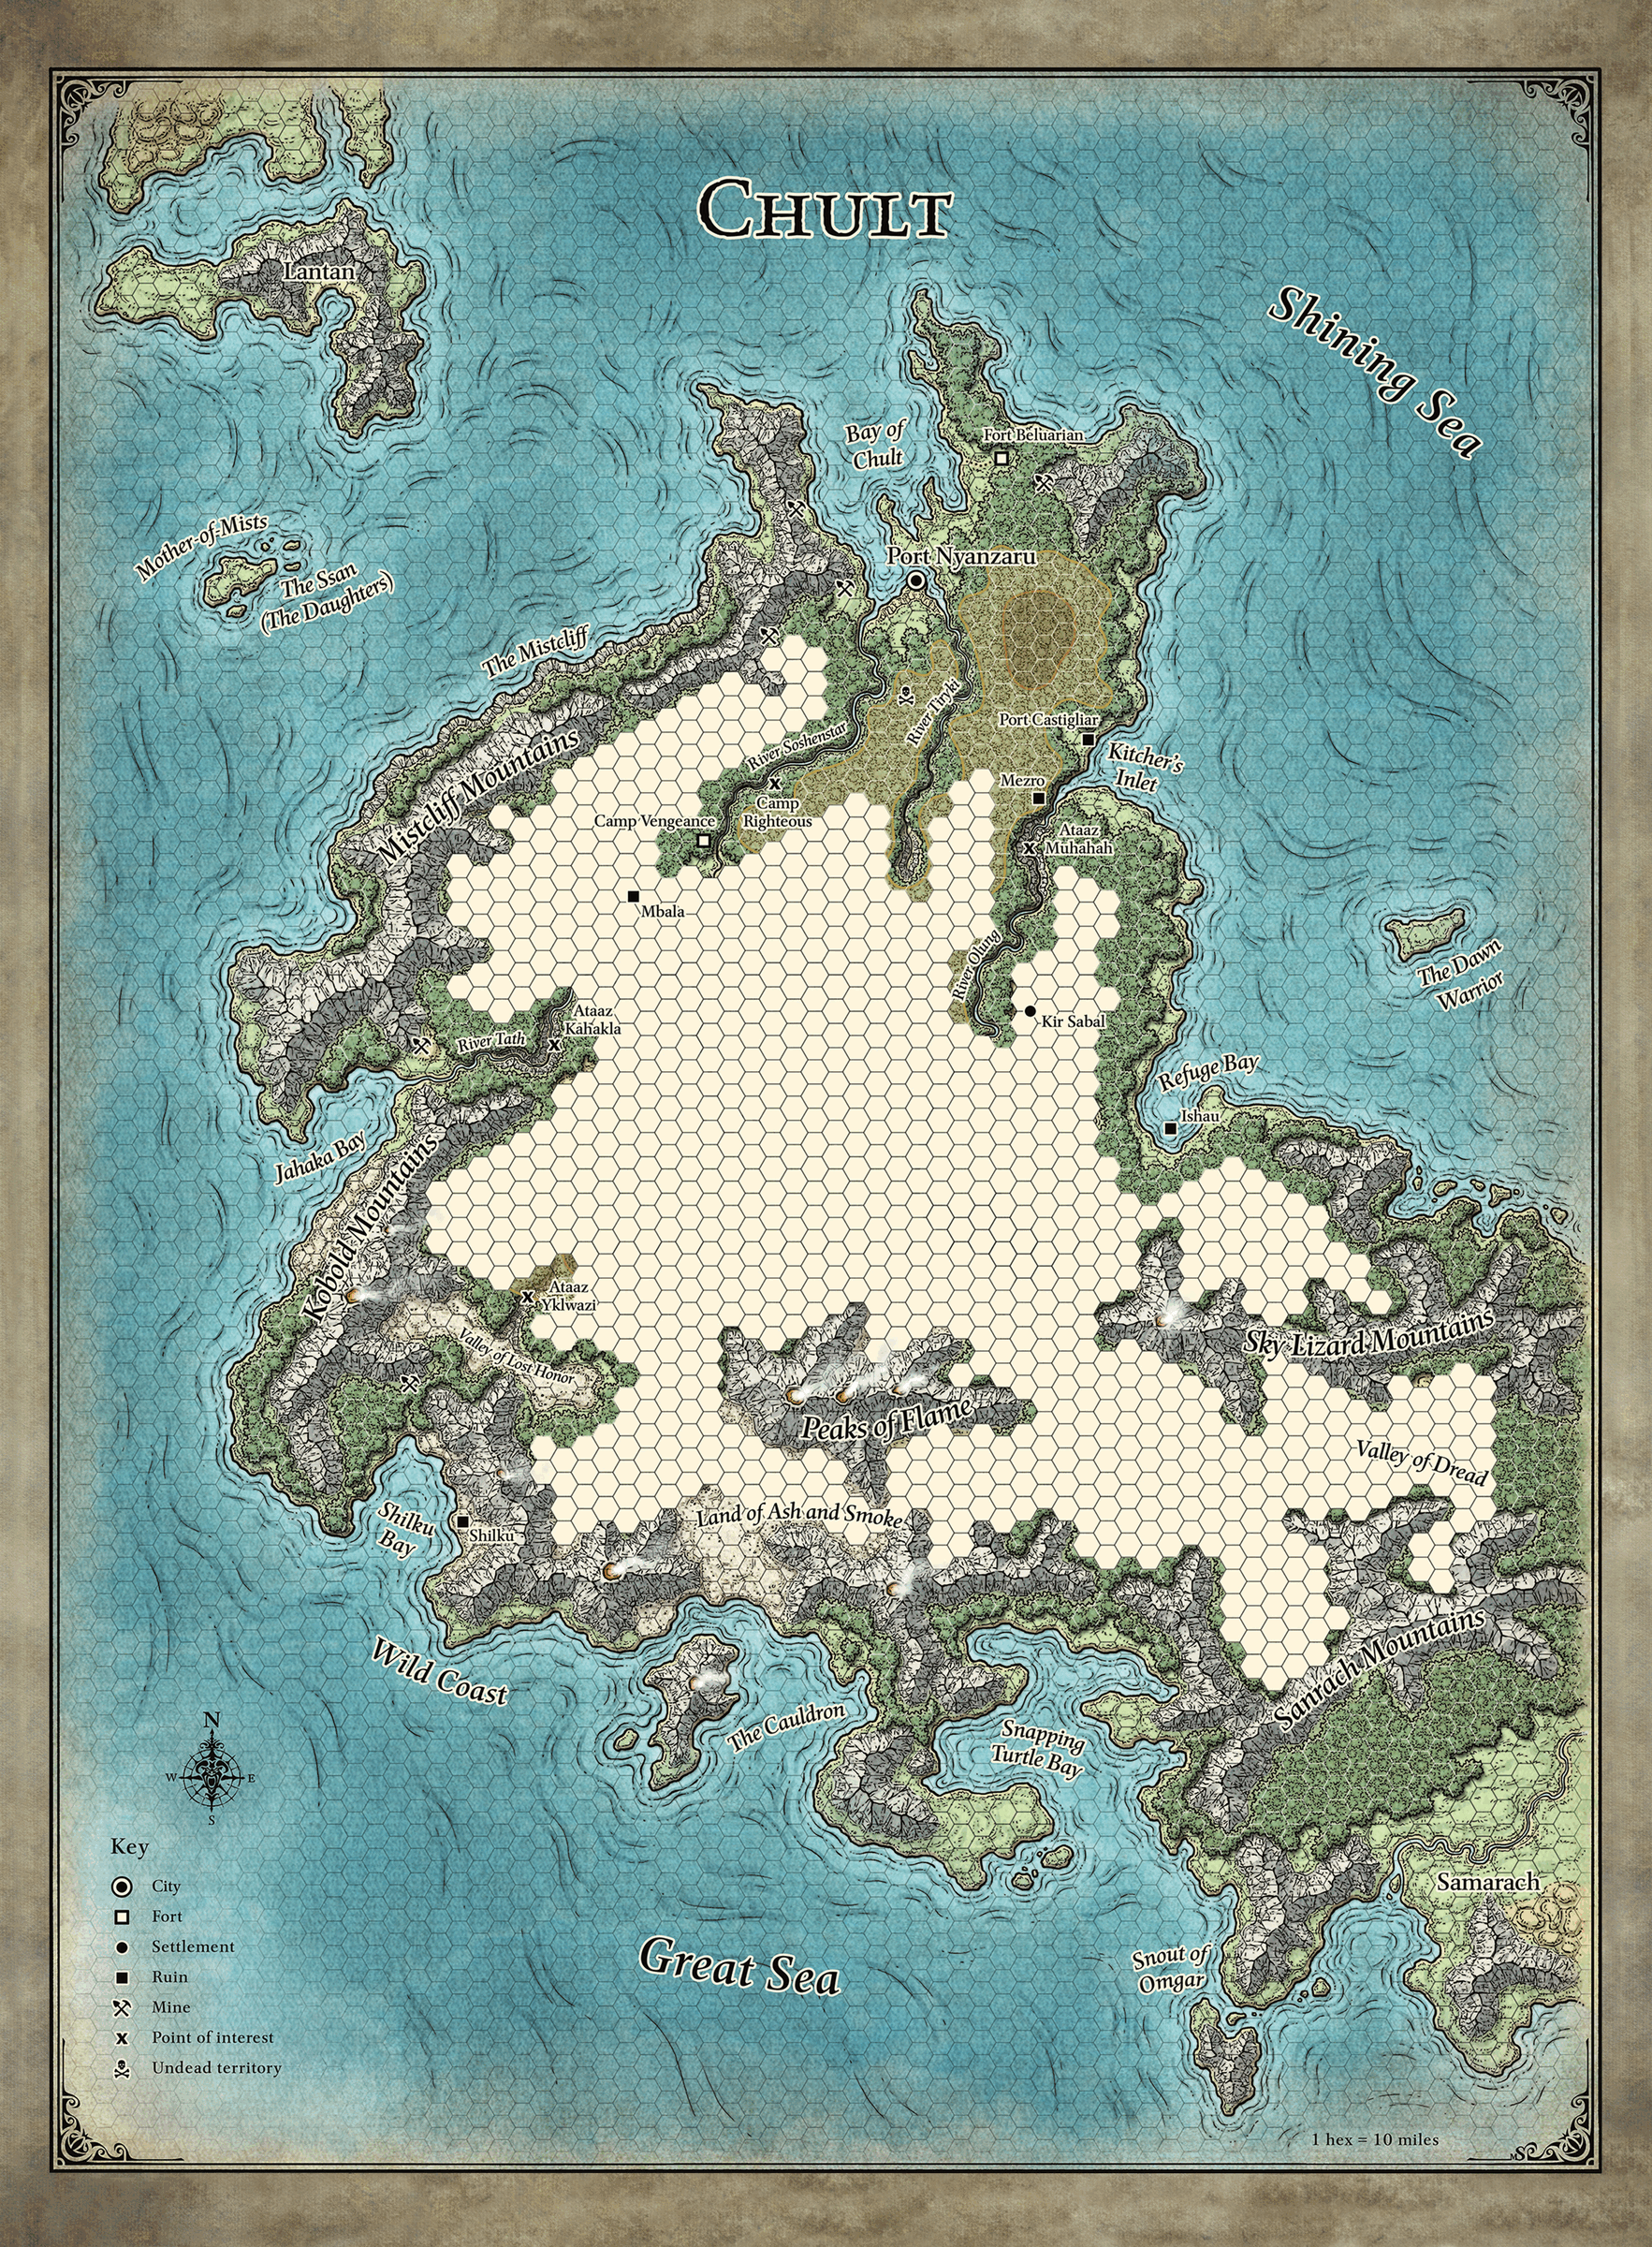
\includegraphics[width=148.5mm,height=210mm]{chult-map-player-version.png}};

  % Fond parchemin - moitié droite.
  \node[anchor=south west,inner sep=0pt]
    at ([xshift=148.5mm]current page.south west)
    {
\includegraphics[width=148.5mm,height=210mm]{fond_parchemin.png}};

  % ---------------------------------------------------------------------------
  % REPÈRES
  % ---------------------------------------------------------------------------
  % Position initiale déterminée à partir du screenshot fourni.
  % Elle reste volontairement facile à ajuster après une première compilation.
    \MapMarker{1}{0.403}{0.680} % Vorn

  % ---------------------------------------------------------------------------
  % LÉGENDE
  % ---------------------------------------------------------------------------
  \node[anchor=north west,text=markertext,font=\bfseries\LARGE]
    at ([xshift=158mm,yshift=191mm]current page.south west) {Chult};

  \node[anchor=north west,text=markertext!80,font=\itshape\small]
    at ([xshift=158mm,yshift=181mm]current page.south west)
    {Lieux découverts par le groupe};

  \node[anchor=west,text=markertext,font=\large]
    at ([xshift=158mm,yshift=165mm]current page.south west)
    {\LegendNumber{1}\hspace{2mm} Vorn};

\end{tikzpicture}
\null
\end{document}
